\documentclass[conference]{IEEEtran}
\IEEEoverridecommandlockouts
\usepackage{cite}
\usepackage{amsmath,amssymb}
\usepackage{graphicx}
\usepackage{booktabs}
\usepackage{array}
\usepackage{xcolor}
\usepackage{url}
\usepackage[hidelinks]{hyperref}
\graphicspath{{figures/}}

% Progress Report 1 (team version), revised for clarity and length.
% Figures are the team's own figures, cut as vector graphics from CS415_LCR_Progress_Report_1.pdf.
% Numbers are copied from script outputs, not typed from memory. Sources:
%   report/generated/*.tex (data, result, look, power, check_s4 macros; retell and intervention tables),
%   docs/generated/LOOK_E3_METRICS.md (Look v4 by kind), docs/generated/LOOK_FORCED_HALLUCINATION_B.md,
%   results/look_small_object_B.json, results/check_s4_B.json.

\begin{document}

\title{Look--Check--Retell: Learning to Use Visual Verification Feedback for Faithful Image Captioning\\[2pt]
\large CS415 Term Project --- Progress Report}

\author{
\IEEEauthorblockN{%
\.{I}brahim G\"{o}zl\"{u}kaya (34528) \quad
Metin Caner Ayd\i{}n (34541) \quad
\.{I}brahim Billurcu (34264)\\
Zeynep Bahar Deniz (34194) \quad
Damla Kemal (34392)}
\IEEEauthorblockA{Faculty of Engineering and Natural Sciences, Saban\c{c}\i{} University, Istanbul, Turkey}
}

\maketitle

\begin{abstract}
Image captioning models sometimes name objects that are not in the image (object hallucination).
Look--Check--Retell (LCR) tries to reduce this in three steps. A frozen BLIP captioner writes a draft;
\emph{Look} uses the captioner's own cross-attention to find where each object word comes from; \emph{Check}
asks a separate frozen detector, OWLv2, whether that object is really there; \emph{Retell} feeds this evidence
back through a small trainable pathway. This report covers the first half of the project on Flickr8k.
Fine-tuning BLIP's decoder raised validation CIDEr from 0.669 to 0.979. BLIP's raw attention finds the right
region for only 12.9\% of claims (against human boxes); an ``attention sink'' correction plus head selection
raises this to 80.4\%. On 300 synthetic word swaps, Look's region hits the real object in 81.7\% of cases,
against 22.3\% for the detector's box for the wrong word. Our current Check (S4) lowers false alarms on correct
\emph{thing} claims from 11.7\% to 3.0\% (automatic reference proxy) while catching more clean synthetic
errors. A first Retell run did not use the content of the evidence, which is why we fixed Look and Check first.
Human evaluation and the final Retell training are next.
\end{abstract}

\begin{IEEEkeywords}
image captioning, object hallucination, cross-attention, open-vocabulary detection, verification feedback
\end{IEEEkeywords}

% =====================================================================
\section{Problem and Motivation}

Modern captioners write fluent sentences, but fluent does not mean correct. A dog holding a frisbee becomes
``a dog playing with a ball''; a park photo gains a bench that is not there. Rohrbach \emph{et
al.}~\cite{rohrbach2018object} called this \emph{object hallucination} and showed that such errors follow the
word statistics of the training captions more than the pixels, and that CIDEr can improve while hallucination
gets worse. For a reader who cannot see the image, such as a screen-reader user, a wrong object is worse than a
missing one, because nothing in a fluent sentence says which word to doubt.

\textbf{Problem statement.} An \emph{object claim} is a concrete noun in a caption that belongs to a fixed
vocabulary $V$ (e.g., \emph{dog}, \emph{ball}, \emph{water}). A claim is \emph{incorrect} if the object is not
visible or a different object got its name. Given an image and a draft caption, we want a new caption with
fewer incorrect claims, without losing correct claims or general caption quality.

\textbf{Main idea and research question.} LCR is a two-pass captioner (Fig.~\ref{fig:pipeline}): draft, Look,
Check, Retell. The detector is not perfect either, so the system has to learn when to trust the evidence. We
ask: \emph{can a captioner learn to use noisy, object-specific verification evidence, while ignoring misleading
evidence, when the checked regions are chosen by its own attention?} The proposal turned this into seven
hypotheses (H1, H1b, H2--H6), restated in Section~\ref{sec:eval}.

\textbf{Scope.} We check only object identity and presence; actions, colours, counts, gender and age are out
of scope. All person words form one class \emph{person}, checked only for presence, because detector-based
gender and age judgements are unreliable and raise fairness concerns~\cite{hendricks2018women}.

\begin{figure*}[t]
\centering
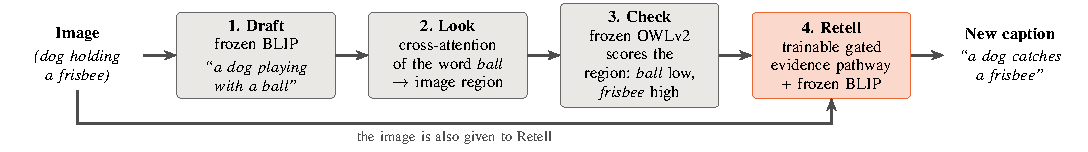
\includegraphics[width=\textwidth]{fig1_pipeline}
\caption{Look--Check--Retell. Grey blocks are frozen; only the orange evidence pathway is trained. The example
is illustrative. Retell receives the image and the verification records; since the detector can be wrong,
Retell must learn when to use the evidence.}
\label{fig:pipeline}
\end{figure*}

% =====================================================================
\section{Related Work}
\label{sec:related}

\textbf{Captioning models.} Early captioners paired a CNN encoder with an LSTM decoder: Show and
Tell~\cite{vinyals2015show} and Karpathy and Fei-Fei~\cite{karpathy2015deep}. Show, Attend and
Tell~\cite{xu2015show} added visual attention, so that each word looks at different image locations; Look
builds on this idea. Bottom-up and top-down attention~\cite{anderson2018bottom} used detector regions, and
Neural Baby Talk~\cite{lu2018neural} filled caption slots with detected object names. After the
Transformer~\cite{vaswani2017attention} and the Vision Transformer~\cite{dosovitskiy2021image}, captioning moved
to vision--language pre-training: CLIP~\cite{radford2021learning} learned a shared image--text space,
BLIP~\cite{li2022blip} pre-trains an image encoder and a text decoder with explicit cross-attention, and
BLIP-2~\cite{li2023blip2} and LLaVA~\cite{liu2023visual} connect frozen encoders to large language models. We
use BLIP-base because it fits on one GPU and its cross-attention is easy to read.

\textbf{Measuring hallucination.} BLEU~\cite{papineni2002bleu}, METEOR~\cite{banerjee2005meteor},
CIDEr~\cite{vedantam2015cider} and SPICE~\cite{anderson2016spice} compare a caption with references;
CLIPScore~\cite{hessel2021clipscore} uses CLIP instead. None counts wrong objects.
CHAIR~\cite{rohrbach2018object} counts generated objects missing from COCO~\cite{lin2014microsoft}
annotations, POPE~\cite{li2023evaluating} asks yes/no object questions, and ALOHa~\cite{petryk2024aloha}
extends CHAIR to an open vocabulary. Dai \emph{et al.}~\cite{dai2023plausible} show that pre-training
objectives affect hallucination. All of these need object annotations; Flickr8k~\cite{hodosh2013framing} has
only five captions per image that do not mention every object, so human judgement is our main measure.

\textbf{Correcting captions with detectors.} CRN~\cite{feng2020cascaded} learns to replace inaccurate words
with detected objects; ReFrame~\cite{adhikary2024reframe} applies rule-based corrections;
Woodpecker~\cite{yin2024woodpecker} and Visual Fact Checker~\cite{ge2024visual} let a language model rewrite
or write captions using expert vision tools; HALC~\cite{chen2024halc} changes decoding with an
open-vocabulary detector. OWL-ViT~\cite{minderer2022simple} and OWLv2~\cite{minderer2023scaling} score image
regions against any text query, like GLIP~\cite{li2022grounded} and Grounding DINO~\cite{liu2024grounding}. We
use OWLv2 because its region features can be cached once and scored against any later query.

\textbf{Learned editing, feedback and decoding.} Show, Edit and Tell~\cite{sammani2020show} edits an existing
caption; LURE~\cite{zhou2024analyzing} trains a revisor on synthetically corrupted descriptions but receives no
object-specific detector feedback; VOLCANO~\cite{lee2024volcano} revises using self-written feedback;
HELPD~\cite{yuan2024helpd} uses object- and sentence-level feedback in training; Biten \emph{et
al.}~\cite{biten2022let} feed global object labels, which do not verify individual claims.
OPERA~\cite{huang2024opera} and visual contrastive decoding~\cite{leng2024mitigating} change token selection
without training.

\textbf{Attention as localisation.} Attention is not automatically an explanation~\cite{jain2019attention};
Grad-CAM~\cite{selvaraju2017grad} and Transformer relevance~\cite{chefer2021generic} are alternatives. Vision
Transformers dump attention on uninformative tokens (artefacts fixed with registers~\cite{darcet2024vision});
language models show the related ``attention sink''~\cite{xiao2024efficient}. We found the same in BLIP
(Section~\ref{sec:exp-look}). Zhang \emph{et al.}~\cite{zhang2025mllms} show that multimodal models often
attend to the right region even when their answer is wrong, while Geigle \emph{et al.}~\cite{geigle2024does}
find that grounding objectives alone barely reduce hallucination. Flickr30k
Entities~\cite{plummer2015flickr30k} provides human boxes for measuring localisation.

\textbf{Adding inputs to a frozen model.} Flamingo~\cite{alayrac2022flamingo} inserts cross-attention layers
whose $\tanh$ gates start at zero, so the model initially behaves exactly like the original; adapters~
\cite{houlsby2019parameter}, LoRA~\cite{hu2022lora} and LLaMA-Adapter~\cite{zhang2024llama} are related.
Retell follows Flamingo.

\textbf{Research gap.} Table~\ref{tab:prior} compares the closest work. In the work we reviewed, no method
trains a captioner to use external, claim-specific evidence whose regions are chosen by the captioner's own
attention. This does not prove novelty; our contribution is to build this and test whether the captioner uses
correct and incorrect evidence selectively.

\begin{table}[t]
\caption{Closest prior work. \emph{External}: claim-specific evidence from a separate model at test time.
\emph{Own att.}: the captioner's attention selects the checked region.}
\label{tab:prior}
\centering\footnotesize\setlength{\tabcolsep}{2.5pt}
\begin{tabular}{@{}lcccl@{}}
\toprule
Method & Learned & External & Own att. & Output \\
\midrule
CRN~\cite{feng2020cascaded} & yes & yes & no & word swap \\
ReFrame~\cite{adhikary2024reframe} & no & yes & no & rule fix \\
Woodpecker~\cite{yin2024woodpecker}, VFC~\cite{ge2024visual} & no & yes & no & LLM rewrite \\
HALC~\cite{chen2024halc} & no & yes & no & decoding \\
Show-Edit-Tell~\cite{sammani2020show}, LURE~\cite{zhou2024analyzing} & yes & no & no & editing \\
VOLCANO~\cite{lee2024volcano} & yes & no & no & self-feedback \\
HELPD~\cite{yuan2024helpd} & yes & no & no & feedback \\
Biten \emph{et al.}~\cite{biten2022let} & yes & no & no & label input \\
\midrule
\textbf{LCR (ours)} & yes & yes & yes & regeneration \\
\bottomrule
\end{tabular}
\end{table}

% =====================================================================
\section{Work So Far (a): Design Decisions and Justification}
\label{sec:design}

For each main choice we say what we chose, the alternative, and why. Table~\ref{tab:design} summarises the
decisions and Table~\ref{tab:names} lists the short names used below.

\begin{table}[t]
\caption{Short names used in this report.}
\label{tab:names}
\centering\footnotesize
\begin{tabular}{@{}>{\raggedright\arraybackslash}p{1.1cm}>{\raggedright\arraybackslash}p{6.7cm}@{}}
\toprule
Name & Meaning \\
\midrule
A, B & The two halves of the Flickr8k training images (3,000 each). \\
B0 & Draft captioner: BLIP, decoder fine-tuned on A, then frozen. \\
B0+ & Retell with no evidence (null token only); effect of extra training data. \\
B1 & Rule: replace each contradicted word with Check's alternative. \\
B2 & Retell with image-level detector tags instead of claim records. \\
B3 & Retell with the detector's best box for the word instead of Look's. \\
LCR & The full system (``Ours''). \\
v1--v4 & Look versions (v1: proposal's rule; v4: current). \\
S2--S4 & Check versions (S4: current). \\
RUOR & Share of claims no reference caption mentions (proxy). \\
HICR & Human-verified incorrect claim rate (main measure; pending). \\
\bottomrule
\end{tabular}
\end{table}

\subsection{Held-Out Drafts and Frozen Features}
The 6,000 training images are split by a fixed seed into halves A and B (3,000 each, no overlap). BLIP is
fine-tuned on A and frozen; its drafts on B are used to choose all Look and Check settings and to train Retell.
Validation is used for reporting (one exception, Section~\ref{sec:exp-draft}); the test split has not been
opened. A second run will swap A and B (the \emph{reversed split}). \emph{Why:} a captioner describes its own
training images unusually well, so drafts on them would almost never be wrong and Retell would never learn to
fix anything.

We fine-tune only BLIP-base's~\cite{li2022blip} 12-layer text decoder and keep the ViT encoder frozen.
\emph{Why:} patch features then never change, so we compute them once; every later stage and every baseline
reads the same features, the attention grid has a fixed geometry, and fine-tuning takes about five minutes on
one GPU.

\subsection{Claim Vocabulary}
$V$ has 169 classes and 316 word forms, chosen by hand from nouns that appear at least 30 times in the
training captions; synonyms share a class (\emph{bicycle}/\emph{bike}). Each class has a \emph{kind}: person
(1), thing (130) or stuff (38, e.g., \emph{water}, \emph{snow}). A word is a claim if it is tagged as a noun,
maps to a class, and does not modify another vocabulary noun (\emph{water bottle} is a bottle); fixed
expressions (``looks at the camera'', ``hot dog'') are skipped. \emph{Why:} WordNet~\cite{miller1995wordnet}
groups filed \emph{table} and \emph{forest} under groups; a fixed list also enforces the fairness rule. The
kind label is our addition: a box detector cannot localise \emph{snow} the way it localises a \emph{frisbee}.

\subsection{Look: From Attention to a Region}
\label{sec:design-look}
We replay the draft with teacher forcing and read the cross-attention at the step that predicts the first word
piece of each claim, giving a $24\times24$ map.

\textbf{Sink correction and heads.} Raw attention puts most weight on the same background patches for every
word. We subtract the caption-wide average map, keep positive values and normalise, leaving the part specific
to this word (related to~\cite{darcet2024vision,xiao2024efficient}; the caption-average version is ours). We
use four heads (two in layer 9, two in layer 10) chosen on half B with a label-free criterion, and refine
person regions with SAM~\cite{kirillov2023segment} masks.

\textbf{Region ranking.} Among OWLv2's 100 proposals, each box $b$ with attention mass $m_A(b)$ is ranked by
\begin{equation}
r(b) = \frac{m_A(b)}{a(b)^{\alpha}}\, o(b)^{\gamma},
\label{eq:rank}
\end{equation}
where $a(b)$ is the box area fraction and $o(b)$ the detector's objectness. With $\alpha=0.5$, large boxes are
not rewarded for size and tiny boxes are not over-rewarded. Look keeps the top three boxes. The detector's
score for the claimed word is not used, so Look's choice is independent of what the detector thinks the object
is.

\textbf{Change from the proposal.} The proposal's rule (v1) used raw last-$k$-layer attention, one box by
excess attention mass, a $2\times2$-patch minimum size, and a ``no suitable region'' option. The sink
correction and Eq.~\eqref{eq:rank} raised region accuracy from 12.9\% to 75.3\%; three boxes without the size
minimum raised small-object coverage from 4.9\% to 55.6\%; the abstention signals were close to chance
(Section~\ref{sec:exp-wrong}); and the proposal's gradient relevance map~\cite{chefer2021generic} scored 2.4
points below the sink-corrected map on half B.

\subsection{Check: Verifying the Region with OWLv2}
\label{sec:design-check}
For each OWLv2~\cite{minderer2023scaling} proposal we cache the box, objectness, a 512-d class embedding
$\mathbf{z}_p$, and the detector's per-box shift $\beta_p$ and scale $\gamma_p$, so the score for any class $c$
with text embedding $\mathbf{q}_c$ is one dot product:
\begin{equation}
\ell_p(c) = \gamma_p\,(\mathbf{z}_p^{\top}\mathbf{q}_c + \beta_p).
\label{eq:owl}
\end{equation}
\emph{Why:} the proposal cached only $\mathbf{z}_p$, but reading the detector code showed that the scores
cannot be reproduced without $\beta_p$ and $\gamma_p$.

\textbf{Rival-aware evidence.} A wrong word usually names something similar (\emph{dog}/\emph{cat},
\emph{shirt}/\emph{jacket}), so we compare the claim with its rivals on the same box. Each class belongs to at
most one hand-made set $S(c)$ of mutually exclusive names, and
\begin{equation}
v_p(c) = \ell_p(c) - w \max\Bigl(0,\ \max_{j\in S(c)} \ell_p(j) - \ell_p(c)\Bigr),\quad w=2.
\label{eq:rival}
\end{equation}

\textbf{Five actions.} Let $R_c$ be the best $v_p(c)$ over Look's three boxes, $X_c$ the best over the whole
image, and $\tau_c$ a per-class threshold. \emph{Keep} if $R_c\ge\tau_c$; \emph{keep elsewhere} if
$R_c<\tau_c\le X_c$ (present, just not where the captioner looked); \emph{replace} if $X_c<\tau_c$ and a rival
on Look's top box passes its own threshold and beats the claim; \emph{remove} if $X_c<\tau_c$ and no rival
qualifies; \emph{skip} if there is no threshold, no region, or a fixed expression. Among qualifying rivals we
pick the one highest relative to its own class centre (median score where the class is likely present); this
\emph{centred substitute rule} stops classes that the detector always scores high from winning by default.
\emph{Why:} the proposal used three verdicts and already said that not finding an object in one region does
not mean it is absent; the five actions apply this directly, since a claim is contradicted only if it is weak
everywhere. Absence is an image-level question; Look's job is to say \emph{which} object the word refers to,
so the substitute is read from the right box.

\textbf{Thresholds.} The previous Check (S2) applied one shared threshold to normalised scores and contradicted
about 32\% of correct clothing claims. S4 picks a threshold per class,
\begin{equation}
\tau_c = \arg\max_{\tau}\ \bigl[F_u(\tau) - \lambda F_p(\tau)\bigr],
\label{eq:tau}
\end{equation}
where $F_p$, $F_u$ are the score distributions of images whose references mention $c$ at least twice (likely
present) or never (likely absent). We chose $\lambda=2.5$ to keep false alarms on supported thing claims at
or below 3\%. These labels come from references, so this calibration is interim until human labels exist.

\begin{table*}[t]
\caption{Summary of the main design decisions. ``(change)'' marks decisions that refine or replace the
original proposal.}
\label{tab:design}
\centering\footnotesize
\begin{tabular}{@{}>{\raggedright\arraybackslash}p{1.5cm}>{\raggedright\arraybackslash}p{5.0cm}>{\raggedright\arraybackslash}p{3.9cm}>{\raggedright\arraybackslash}p{6.2cm}@{}}
\toprule
Part & Our choice & Alternative & Reason \\
\midrule
Data & Split Flickr8k train into halves A and B; captioner trained on A, Retell trained on B & Train both on
all of train & The captioner makes realistic mistakes only on images it was not fine-tuned on. \\
Captioner & Fine-tune only BLIP's text decoder; image encoder frozen and features cached (change) & Fine-tune
all of BLIP & Every system sees identical image features; training takes minutes on one GPU. \\
Vocabulary & 169 hand-curated classes, three kinds: person / thing / stuff (change) & Automatic WordNet
groups & WordNet groups were unusable; a detector handles \emph{water} very differently from
\emph{frisbee}. \\
Look map & Subtract caption-wide average attention (``sink correction'') and use four selected heads
(change) & Proposal: raw attention averaged over the last $k$ layers, $k\in\{1,4,12\}$ & Raw attention piles
up on the same background patches for every word (Sec.~\ref{sec:exp-look}). \\
Look region & Rank detector proposals by attention density; keep top three; no ``no region'' option
(change) & Proposal: one box by excess attention mass, at least $2\times2$ patches, abstain below a threshold
& Top three catches more true objects; abstention signals were close to chance (Sec.~\ref{sec:exp-wrong}). \\
Check scores & Cache OWLv2 region features and its per-box scale/shift (change) & Cache only the features &
Without scale and shift the detector's scores cannot be reproduced. \\
Check rule & Rival-aware evidence, one threshold per class, five actions (change) & Proposal: three verdicts.
S2: five actions but one shared threshold on normalised scores & The shared threshold contradicted 32\% of
correct clothing claims; five actions separate ``not here'' from ``nowhere''. \\
Retell & Zero-initialised $\tanh$-gated cross-attention in the upper six decoder layers & Fine-tune the
whole decoder & Training starts exactly from the draft model, and gate values show how much evidence is
used. \\
Training data & Synthetic label swaps using the captioner's own next-best word (change) & Proposal: a
frequently co-occurring wrong noun (e.g., \emph{frisbee} $\to$ \emph{ball}) & Real errors are rare; the
runner-up word is the mistake this captioner was closest to making. \\
Evaluation & Choose settings on B, report on validation, test only once; paired claim-level test & Tune on
validation; unpaired test & Keeps validation honest; the paired test needs far fewer annotated claims
(Table~\ref{tab:power}). \\
\bottomrule
\end{tabular}
\end{table*}

\subsection{Retell: Gated Evidence Pathway}
\label{sec:design-retell}
Each checked region becomes one evidence token
$\mathbf{t} = \mathrm{LN}\bigl(W_c\mathbf{w}_c + W_a\mathbf{w}_a + f([\mathbf{z}_r;\mathbf{g}]) +
\mathbf{e}_{\text{action}}\bigr)$, where $\mathbf{w}_c,\mathbf{w}_a$ are BLIP's own word embeddings of the
claimed and alternative label, $f$ is a small MLP over the region feature $\mathbf{z}_r$ and scores/geometry
$\mathbf{g}$, and $\mathbf{e}$ embeds Check's decision; a learned null token is always added. Before each of the
upper six decoder layers we insert a Flamingo-style~\cite{alayrac2022flamingo} block:
\begin{align*}
\mathbf{h} &\leftarrow \mathbf{h} + \tanh(\alpha_1)\,\mathrm{CrossAttn}\bigl(\mathrm{LN}(\mathbf{h}),
T\bigr),\\
\mathbf{h} &\leftarrow \mathbf{h} + \tanh(\alpha_2)\,\mathrm{FF}\bigl(\mathrm{LN}(\mathbf{h})\bigr),
\end{align*}
with evidence tokens $T$ and $\alpha_1=\alpha_2=0$ at the start (23.5\,M trainable parameters; BLIP and OWLv2
frozen). \emph{Why:} since $\tanh(0)=0$ the system starts exactly as the draft captioner and the gate values
show whether evidence is used; BLIP's own embeddings put ``the alternative is \emph{frisbee}'' in a language
the decoder already understands; object words are decided late, so only the upper layers get the pathway,
halving its size for 3,000 training images. Retell does not see the draft sentence, only the records, so
changing a record and watching the output cleanly tests evidence use.

\textbf{Synthetic corruption.} Real draft errors are rare, so with probability $\rho=0.15$ we replace a
training claim with a wrong label, recompute its scores with Eq.~\eqref{eq:owl}, and keep the true label as
the alternative, similar to LURE~\cite{zhou2024analyzing}. \emph{Change from the proposal:} the wrong label is
the captioner's own next-best word instead of a co-occurring noun, i.e., the mistake it was closest to making.

\textbf{Baselines.} All are defined in the proposal (Table~\ref{tab:names}). B0+, B2 and B3 are matched
controls: same architecture, optimiser and updates as LCR, differing only in their input. B2 (image-level tags,
inspired by~\cite{biten2022let}) tests whether claim-specific evidence beats a global tag list; B3 tests
whether the captioner's attention helps; B0+ measures the gain from Retell's 3,000 extra training images alone,
so every claim about evidence is made against B0+, not only B0.

\subsection{Evaluation Design}
\label{sec:eval}
\textbf{Hypotheses (from the proposal).} The main measure is HICR, the share of object claims annotators label
as incorrect. \textbf{H1:} Ours lowers HICR by $\ge$15\% (relative) vs.\ B0, and also vs.\ B0+, while losing at
most 5\% of correct claims per image. \textbf{H1b:} on the 5,000-image COCO Karpathy
test~\cite{karpathy2015deep,lin2014microsoft}, without further training, Ours lowers CHAIR$_i$
\cite{rohrbach2018object} by $\ge$10\% vs.\ B0 and B0+ (COCO's exhaustive annotations allow automatic CHAIR on
many claims). \textbf{H2:} Ours has a higher net repair rate (fixed errors $-$ broken correct claims, over all
draft claims) than B1, with a break rate at most 3 points above B1's. \textbf{H3:} claim records give lower
HICR than B2's tags. \textbf{H4:} correct evidence raises adoption of the correct label by $\ge$25 points vs.\
no evidence, and false evidence is adopted $\ge$25 points less often than correct evidence. \textbf{H5:} CIDEr
within 3\% of B0, SPICE drop $\le$1 point. \textbf{H6:} the lower 95\% CI bound of (Ours $-$ B3) localisation
accuracy is above $-5$ points (superiority only if the whole CI is above 0). All differences need paired
image-level bootstrap 95\% CIs that exclude zero. Annotators label every concrete noun, including nouns outside
$V$, so a system cannot hide errors in unchecked objects. Before human labels exist, a claim is called
\emph{reference-supported} if a reference mentions its class; this is a proxy and labelled as such.

\textbf{Sample size.} Two independent samples would need 7,469 claims per system to detect H1's 15\%
reduction at an 8\% error rate (Table~\ref{tab:power}). Since both systems caption the same images and most
claims do not change, a paired test on \emph{traced} claims (each draft claim followed into the new caption as
fixed, broken or unchanged) is far more efficient: 2,000 claims give about 85\% power. These numbers assume
independent claims (optimistic) and depend on the real error rate, which the pilot will measure. With about
2.27 claims per image, the proposal's maximum $N=400$ test images gives roughly 900 traced claims, below the
1,000-claim column. If the error rate is 8\% or lower, H1 will be hard to establish, and, as the proposal
foresees, COCO CHAIR (H1b) becomes the main factuality evidence.

\begin{table}[t]
\caption{Power analysis for H1 (15\% relative reduction, $\alpha=0.05$). Left: claims per system for an
unpaired test at 80\% power. Right: simulated power of a paired sign test on traced draft claims (1\% of
correct claims broken).}
\label{tab:power}
\centering\footnotesize
\begin{tabular}{@{}lcccc@{}}
\toprule
Draft error & Unpaired & \multicolumn{3}{c}{Paired power at $N$ claims} \\
\cmidrule(l){3-5}
rate & claims & 1,000 & 2,000 & 4,000 \\
\midrule
8\% & 7,469 & 52\% & 85\% & -- \\
5\% & -- & -- & 50\% & 82\% \\
\bottomrule
\end{tabular}
\end{table}

% =====================================================================
\section{Work So Far (b): Experiments and Results}
\label{sec:experiments}

\subsection{Setup and Data}
We use Flickr8k~\cite{hodosh2013framing}: 8,000 images, five captions each, standard 6,000/1,000/1,000 split.
Settings are chosen on half B and results reported on validation unless stated; the test split has not been
read. GPU stages ran on one Colab GPU. Every number is written by a script in our repository. Training
captions average 10.8 words and 2.10 claims; persons are 34.5\% of claims, things 44.8\% and stuff 20.7\%. The
class distribution is very skewed (Fig.~\ref{fig:freq}), one reason a single threshold for all classes did not
work.

\begin{figure}[t]
\centering
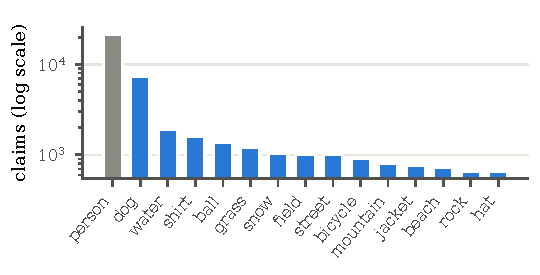
\includegraphics[width=0.85\columnwidth]{fig2_claim_freq}
\caption{The 15 most frequent claim classes in the training captions (log scale). Grey: the person class.}
\label{fig:freq}
\end{figure}

\subsection{Drafting Captioner}
\label{sec:exp-draft}
We fine-tuned BLIP's decoder on half A for three epochs (AdamW~\cite{loshchilov2019decoupled}, learning rate
$2\times10^{-5}$, batch 32). Validation CIDEr peaked after epoch 1 and then slowly dropped while training loss
kept falling (Fig.~\ref{fig:ft}), so we froze the epoch-1 model as B0. This choice used validation CIDEr and is
the one exception to our rule that validation is only for reporting; later checkpoints will be selected on
held-out training images. Fine-tuning mainly adapts style (Table~\ref{tab:caption}): BLEU-4 and CIDEr rise and
drafts mention more objects (2.27 vs.\ 1.84 claims per image), but RUOR does not go down (14.0\% $\to$
15.8\%). A better-scoring captioner is not automatically a more faithful one~\cite{rohrbach2018object}.
METEOR and SPICE need a Java toolkit that was not available and will be added.

\begin{table}[t]
\caption{Caption quality on validation (1,000 images). BLEU-4 $\times100$. RUOR: share of claims no reference
mentions (reference agreement, not a hallucination rate).}
\label{tab:caption}
\centering\footnotesize
\begin{tabular}{@{}lccc@{}}
\toprule
Captioner & BLEU-4 & CIDEr & RUOR (\%) \\
\midrule
BLIP zero-shot & 25.6 & 0.669 & 14.0 \\
BLIP fine-tuned on A (B0) & 32.6 & 0.979 & 15.8 \\
\bottomrule
\end{tabular}
\end{table}

\begin{figure}[t]
\centering
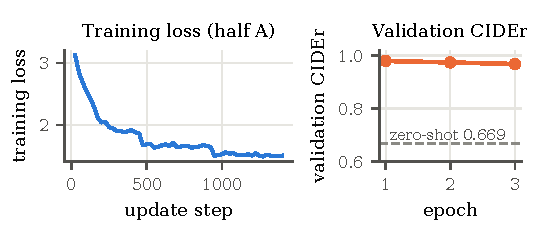
\includegraphics[width=\columnwidth]{fig3_finetune}
\caption{Decoder fine-tuning on half A: training loss (left) and validation CIDEr per epoch (right; dashed:
zero-shot).}
\label{fig:ft}
\end{figure}

\textbf{How good is the reference proxy?} B0 makes 2,272 validation claims; 84.2\% are mentioned by a
reference (person 99.1\%, thing 75.2\%, stuff 79.7\%). For 64.0\% of the 258 unmentioned thing claims, OWLv2
finds the class in the image with a high score, so many are probably real objects the annotators did not
mention. Reference agreement cannot replace human judgement, and the detector separates mentioned from
unmentioned claims well for persons (AUROC 0.86) and things (0.79) but poorly for stuff (0.64).

\subsection{Look: Is Cross-Attention Useful for Finding Objects?}
\label{sec:exp-look}
We compare Look with human boxes from Flickr30k Entities~\cite{plummer2015flickr30k}; 1,795 of the 2,272
validation claims (79.0\%) have one. A box is correct if its IoU with a same-class human box is $\ge$0.5.
Human boxes are used only for measurement and small choices on half B, never for training.

\textbf{Raw attention fails; each fix helps.} With raw attention, only 12.9\% of selected boxes are correct,
and the attention peak lands inside the object only 23.9\% of the time, below random pointing; our first
pipeline run inherited this. Fig.~\ref{fig:look} shows each change: the sink correction raises pointing to
88.3\% and region accuracy to 55.7\%; the ranking of Eq.~\eqref{eq:rank} (v2) gives 75.3\%; tuned smoothing
(v3) 76.1\%; head selection and SAM for persons (v4) 80.4\%, close to the detector's own best box for the
class (82.7\%), although Look never uses the class score. Table~\ref{tab:lookkind} shows that v4 mainly helped
person claims ($+9.3$ points; overall $+4.3$, 95\% CI $[+2.5, +6.1]$). Fig.~\ref{fig:overlays} shows examples.

\begin{figure}[t]
\centering
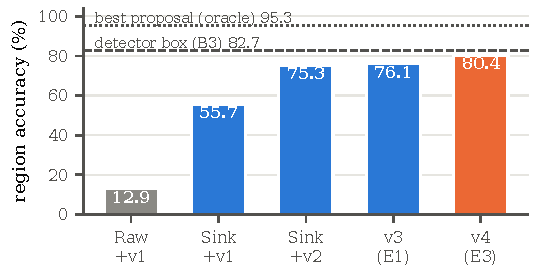
\includegraphics[width=\columnwidth]{fig4_look_steps}
\caption{Look region accuracy on validation against human boxes (1,795 claims). Each bar adds one change:
\emph{Raw+v1} is the proposal's rule on raw attention; \emph{Sink+v1} adds the sink correction;
\emph{Sink+v2} adds the ranking of Eq.~\eqref{eq:rank}; v3 adds tuned smoothing; v4 adds head selection and
SAM for persons (E1, E3: the two tuning rounds on half B). Dashed: the detector's best box for the claimed
class (uses the class score; Look does not). Dotted: best of all 100 proposals (upper bound).}
\label{fig:look}
\end{figure}

\begin{table}[t]
\caption{Look region accuracy (\%) by claim kind on validation. $\Delta$: v4 $-$ v3 with paired
image-bootstrap 95\% CI.}
\label{tab:lookkind}
\centering\footnotesize\setlength{\tabcolsep}{4.5pt}
\begin{tabular}{@{}lcccc@{}}
\toprule
 & All & Person & Thing & Stuff \\
\midrule
$n$ & 1,795 & 761 & 758 & 276 \\
v3 & 76.1 & 67.1 & 83.8 & 79.7 \\
v4 (current) & \textbf{80.4} & \textbf{76.5} & \textbf{85.1} & 78.3 \\
\midrule
$\Delta$ & $+4.3$ & $+9.3$ & $+1.3$ & $-1.4$ \\
95\% CI & $[2.5, 6.1]$ & $[5.3, 13.1]$ & $[-0.1, 2.9]$ & $[-4.7, 1.7]$ \\
\bottomrule
\end{tabular}
\end{table}

\begin{figure}[t]
\centering
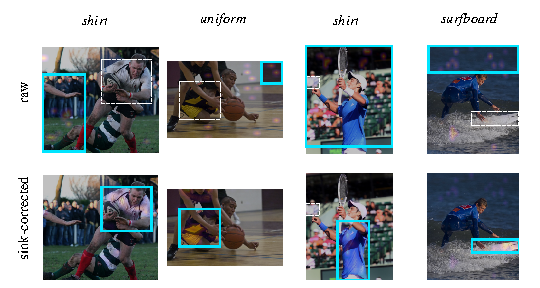
\includegraphics[width=\columnwidth]{fig5_overlays}
\caption{Raw (top) vs.\ sink-corrected (bottom) attention on the same validation claims, first region rule.
Cyan: box chosen from attention; white dashed: detector's best box for the class. Raw attention picks
background (crowd, wall, water); after the correction Look finds the shirt, uniform and surfboard.}
\label{fig:overlays}
\end{figure}

\textbf{Does the map really matter?} On half B, the same ranking with a uniform map reaches only 39.6\%, and
objectness alone 35.9\%, against 74.6\% with the real map. For claims whose image also has a claim of a
different class, using that other claim's map drops accuracy from 74.7\% to 22.1\%, so the map is
word-specific. Masking the image features inside Look's box lowers the claimed word's log-probability by 1.69
on average, against 0.98 for a random mask of the same size (paired difference 0.70, 95\% CI $[0.62, 0.79]$).
On half B, the top three boxes cover the true object for 93.3\% of claims, and small-object coverage rose from
4.9\% to 55.6\% of 162 claims once the minimum-size filter was removed.

\subsection{Look on Wrong Words}
\label{sec:exp-wrong}
When the caption names the wrong object, does Look still point at the object the word refers to? We created
300 misidentified claims on half B by swapping an object word and teacher-forcing the new caption
(Fig.~\ref{fig:wrong}). At the step that predicts the word, Look's top box hits the true object in 81.7\% of
cases (top three: 91.0\%); the detector's box for the wrong word (B3) only 22.3\%, because it searches for the
wrong object. This is the clearest evidence so far for the proposal's central idea: the captioner's attention
points to the right place even when its word is wrong~\cite{zhang2025mllms}. It is also why Check reads
substitutes from Look's top box. Reading one step later, after the wrong word is in the input, drops to
36.3\%. For 251 invented objects (compared with real objects added at the same sentence position), attention
statistics such as concentration and entropy were near chance (AUROC 0.44--0.57): attention cannot tell
whether an object exists, so absence is left to Check at the image level.

\begin{figure}[t]
\centering
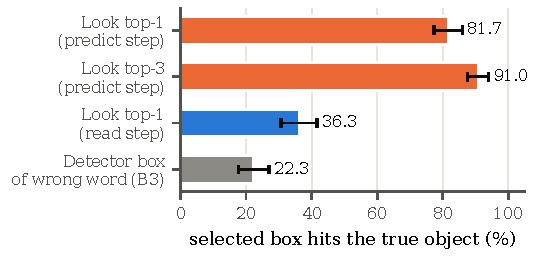
\includegraphics[width=\columnwidth]{fig6_wrong_words}
\caption{Misidentified claims on half B ($n=300$ synthetic swaps): how often the selected box hits the real
object. \emph{Predict step}: attention while the word is predicted; \emph{read step}: one step later. Error
bars: image-level bootstrap 95\% CI.}
\label{fig:wrong}
\end{figure}

\subsection{Check: Calibrated Verification}
\label{sec:exp-check}
\textbf{First attempt.} With fixed thresholds from detection practice ($\tau_s=0.2$, $\tau_c=0.05$) and
raw-attention regions, only 9.5\% of claims were supported and 30.3\% contradicted, although most claims are
correct. The rule baseline B1 then changed 689 words; by the reference proxy only 24 fixed an unsupported claim
and 409 broke a supported one.

\textbf{Current Check (S4).} Without human labels, we test Check on half B with five-fold cross-validation over
images. The \emph{false-alarm rate} is the share of reference-supported claims contradicted; the \emph{swap
test} replaces correct claims with wrong labels (2,401 swaps, 834 ``clean'' swaps to a mutually exclusive name)
and counts how many are caught. Table~\ref{tab:check} compares S4 with S2 (five actions, one shared threshold)
and S3 (thresholds from clean positives only, which met the false-alarm target but caught far fewer swaps).
S4 cuts false alarms on correct thing claims from 11.7\% to 3.0\% and on clothing from 32.0\% to 4.1\%, catches
more clean swaps (80.8\% vs.\ 55.2\%) and about the same share of all swaps (55.5\% vs.\ 55.9\%). Its
substitutes are the true label 91.2\% of the time (S2: 68.9\%). Both new parts help: without the rival term,
clean detection falls to 62.9\%; without the centred substitute rule, substitute accuracy falls to 85.9\%.
Across $\lambda$ (Fig.~\ref{fig:tradeoff}), S2, S3 and the no-rival version all lie below S4's curve. An
exploratory analysis gave only about 71\% substitute accuracy when the substitute was not read from Look's box.

S4 also has costs: more false alarms on stuff (5.4\% vs.\ 1.6\%) and fewer caught swaps between clothing names
(48.4\% vs.\ 62.6\%), where the detector itself confuses \emph{shirt} and \emph{sweater}. On all 4,594
non-person B claims, S4 keeps 4,024, keeps 287 elsewhere, skips 64, removes 167 and replaces 52. These are proxy
and synthetic results on the same B folds used to design S4; only human labels can tell how often its real
interventions are right.

\begin{table}[t]
\caption{Check on half B (5-fold, out-of-fold). \emph{False alarms}: share of reference-supported claims
contradicted. \emph{Swaps}: synthetic label swaps caught. \emph{Subst.}: share of replaced swaps whose
substitute is the true label. All are automatic proxies.}
\label{tab:check}
\centering\footnotesize\setlength{\tabcolsep}{2.4pt}
\begin{tabular}{@{}lccccc@{}}
\toprule
 & \multicolumn{2}{c}{False alarms (\%) $\downarrow$} & \multicolumn{2}{c}{Swaps caught (\%) $\uparrow$} &
Subst. (\%) \\
\cmidrule(lr){2-3}\cmidrule(lr){4-5}
System & thing & clothing & clean & all & $\uparrow$ \\
\midrule
S2 (previous) & 11.7 & 32.0 & 55.2 & 55.9 & 68.9 \\
S3 (positive-anchored) & 3.8 & 4.6 & 24.2 & 26.1 & 85.2 \\
\textbf{S4 (current)} & \textbf{3.0} & \textbf{4.1} & \textbf{80.8} & 55.5 & \textbf{91.2} \\
\midrule
S4 w/o rival term & 2.8 & 5.5 & 62.9 & 47.0 & 93.1 \\
S4 w/o centred subst. & 3.0 & 4.1 & 80.8 & 55.5 & 85.9 \\
\bottomrule
\end{tabular}
\end{table}

\begin{figure}[t]
\centering
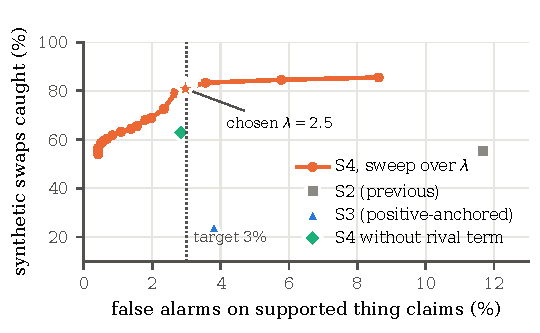
\includegraphics[width=\columnwidth]{fig8_tradeoff}
\caption{False alarms on correct thing claims vs.\ clean synthetic swaps caught (half B). The orange curve
sweeps $\lambda$ in Eq.~\eqref{eq:tau}; the star is the chosen $\lambda=2.5$.}
\label{fig:tradeoff}
\end{figure}

\subsection{Retell: First Training Run}
\label{sec:exp-retell}
We trained Retell and the matched controls once each before Look and Check were fixed (raw or sink-corrected
attention, provisional thresholds). These runs test that the pipeline trains end to end; they do not test the
hypotheses. Before training, all systems reproduced the B0 drafts exactly on 200 validation images, as
expected from $\tanh(0)=0$.

\textbf{The content of the evidence was not used.} All trained systems, including B0+ without evidence, reach
almost the same CIDEr (0.981--0.991) and change about the same share of captions (64--65\%;
Table~\ref{tab:retell}), so the gain over B0 comes from the extra training images. Masking all evidence changes
10.9\% of the captions but leaves the adoption of alternatives unchanged (41.0\%), and replacing each suggested
alternative with a wrong object changes no caption (0.0\%). The pathway reacts to the \emph{presence} of
evidence, not to its \emph{content}. The evidence gates stay almost at zero, while the feed-forward gates grow
the same way with and without evidence (Fig.~\ref{fig:gates}).

\textbf{Diagnosis.} The evidence was mostly noise: during training 60\% of records were uncertain, 31\%
contradicted and only 8\% supported, because the regions were poor and the thresholds wrong; and the decoder
already sees the full image. So we first fixed Look and Check, and extended the evidence token with Check's
action and suggested substitute, which the first version did not encode.

\begin{table}[t]
\caption{First Retell run on validation (historical; provisional thresholds). \emph{Changed}: captions that
differ from the draft. \emph{Alt.}: contradicted claims whose alternative appears in the output. \emph{False
ev.}: captions that change when alternatives are replaced by wrong labels.}
\label{tab:retell}
\centering\footnotesize\setlength{\tabcolsep}{3pt}
\begin{tabular}{@{}lccccc@{}}
\toprule
System & BLEU-4 & CIDEr & Changed & Alt. & False ev. \\
 & & & (\%) & (\%) & (\%) \\
\midrule
B0 (draft) & 32.6 & 0.979 & -- & -- & -- \\
B1 (word replacement) & 27.9 & 0.815 & 40.3 & -- & -- \\
B0+ (no evidence) & 34.0 & 0.983 & 63.6 & -- & -- \\
B2 (image tags) & 34.3 & 0.983 & 64.7 & -- & -- \\
B3 (detector regions) & 34.1 & 0.981 & 64.6 & 26.5 & -- \\
LCR, raw attention & 34.2 & 0.987 & 65.0 & 15.1 & -- \\
LCR, sink attention & 34.3 & 0.991 & 64.1 & 41.0 & 0.0 \\
\bottomrule
\end{tabular}
\end{table}

\begin{figure}[t]
\centering
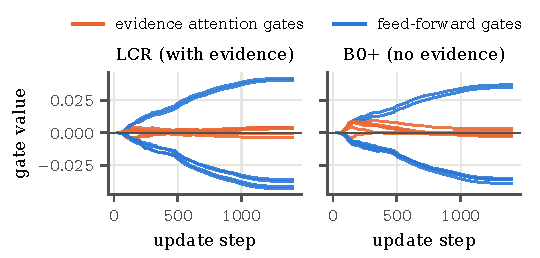
\includegraphics[width=\columnwidth]{fig9_gates}
\caption{Gate values in the first Retell run. Orange: evidence cross-attention gates; blue: feed-forward gates.
The evidence gates barely move; the feed-forward gates behave the same without evidence (B0+).}
\label{fig:gates}
\end{figure}

% =====================================================================
\section{Summary and Next Steps}
\label{sec:conclusion}

\textbf{Work done and results.} We built the data pipeline (A/B split, 169-class vocabulary, cached BLIP and
OWLv2 features with the detector's scale and shift), the draft captioner, Look, Check S4, the Retell pathway
with all matched controls, and the blinded annotation tool. The main findings so far:
\begin{itemize}
\item Higher caption scores did not reduce unmentioned objects (CIDEr 0.669 $\to$ 0.979, RUOR 14.0\% $\to$
15.8\%).
\item Raw cross-attention is unusable for localisation because of attention sinks; a gradient-free correction
plus head selection raises region accuracy from 12.9\% to 80.4\%.
\item For misidentified objects, the captioner's attention finds the true object far more often than the
detector's box for the wrong word (81.7\% vs.\ 22.3\%), but it cannot tell whether an object exists.
\item Per-class, rival-aware verification cuts false alarms on correct thing claims about four times
(automatic proxy).
\item Retell trained on noisy evidence did not use its content; good evidence must come first.
\end{itemize}

\textbf{Changes from the proposal.} Table~\ref{tab:design} marks each change, each justified by a measurement
above. Settings the proposal chose on validation (Look, Check, $\rho$) are now chosen on half B. Still
temporary: Check thresholds are calibrated on reference captions, and B0's epoch was picked on validation.

\textbf{Plan.} Table~\ref{tab:status} gives the status of each work package and the week of the proposal's
12-week schedule in which the remaining ones are planned. The human pilot comes first, because the real draft
error rate, S4's real precision and the test size $N$ all depend on it.

\begin{table}[t]
\caption{Status and plan of the work packages (weeks of the proposal's 12-week schedule).}
\label{tab:status}
\centering\footnotesize\setlength{\tabcolsep}{3pt}
\begin{tabular}{@{}c>{\raggedright\arraybackslash}p{5.4cm}>{\raggedright\arraybackslash}p{1.65cm}@{}}
\toprule
Week & Work package & Status \\
\midrule
1--7 & Pilot run with overlays; BLIP fine-tuned on A; OWLv2 cached; Look v4; Check S4; B1, B2; synthetic
corruption & Done \\
1--7 & Retell pathway, B0+, B3 & Built, trained once \\
8 & Human pilot on half B (two annotators, Cohen's $\kappa$~\cite{cohen1960coefficient}): real error rate,
S4 precision, test size $N$ & Next (tool ready) \\
9 & Retrain LCR, B0+, B2, B3 with v4/S4 records incl.\ Check's action and substitute; $\rho$ ablation; epoch
selection on held-out training images & Next \\
10 & Reversed split; COCO inference, CHAIR$_i$/CHAIR$_s$ (H1b); METEOR, SPICE; B1 with S4 & Next \\
11 & Blinded human evaluation on the test sample; H4 interventions (real, masked, false evidence); H6 & Next
(tool ready) \\
12 & Paired bootstrap statistics; final report & Final \\
\bottomrule
\end{tabular}
\end{table}

\textbf{Risks.} (1) If the real draft error rate is 8\% or lower, H1 may be underpowered even with $N=400$ and
the paired design; as the proposal states, we will say so before the test evaluation, treat COCO CHAIR (H1b)
as the main factuality evidence, and still report HICR with its interval. (2) Retell may still ignore the
evidence; the intervention tests will show this directly, and B3 regions remain a fallback. (3) Annotation is
the largest remaining workload, so the annotation tool is already finished and tested.

\bibliographystyle{IEEEtran}
\bibliography{../refs}

\end{document}
